\chapter{Reconstruction}

The physics objects are detected as a digital signals in each detectors described in Section~\ref{sec:detector}.
Figure~\ref{fig:ParticlePath} shows the diagram of the particles path. What we need in this analysis is the informations of the Bosons and the forward jets, hence these digital signals are finally needed to be reconstructed. In the semi-leptonic process, the Bosons can be seen as its decaying products, leptons and jets. The basical physics objects reconstructed and used in this analysis are Electrons, Muons, Jets, and missing transverse energy (MET). Jets can be seen as a bunch of lots of particles as seen in the calorimeter of the Figure~\ref{fig:ParticlePath}, while muons and electrons can be seen in the detector up to Muon Spectrometer (The MS) and Electromagnetic Calorimeter. 
We need to identify which is the particles or jets we need, starting from the signals in the each detectors. 
Furthermore, all of these physics objets needs to be calibrated, in order to correct the translation from signals to original partons for detector effects.
These reconstruction, identification and the calibration process is described in this chapter.
\begin{figure}[tbp]
\begin{center}
 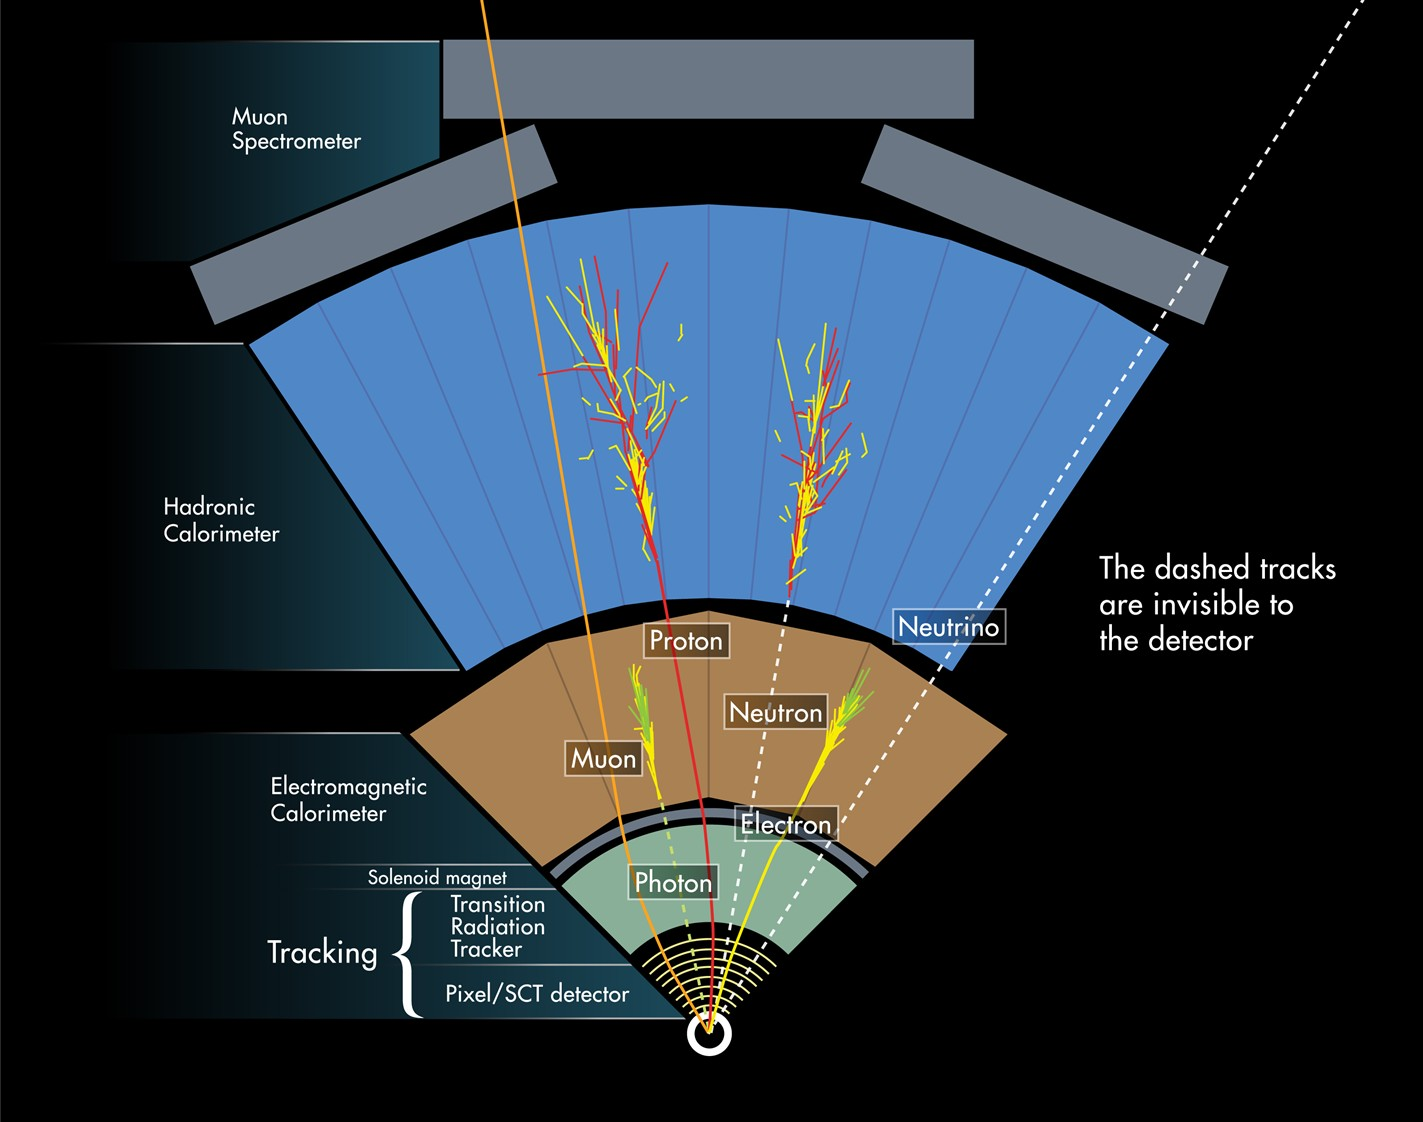
\includegraphics[width=0.80\textwidth,keepaspectratio]{figures/Reconstruction/ParticlePath}
\caption{
Schematics of the particle path
}
\label{fig:ParticlePath}
\end{center}
\end{figure}
\section{Tracks and Vertices}
The track is reconstructed by the Inner Detector (ID). Reconstruction of tracks starts from three-dimentional space points, reconstructed from energy deposits of charged particles, in other words, cluster hits, in the ID components. The track candidate is formed with the sets of space points. The "track score" is calculated and tracks are selected with respect to the scores. Finally the track is fitted and decided. 
Details are described in \cite{PERF-2015-08}.
%put figure here
\section{Clusters}
The reconstruction of the signal from hadrons and jets is based on a three-dimensional topological clustering of individual calorimeter cell signals.
%put figure here
The cluster formation follows cell signal-significance patterns generated by electromagnetic and hadronic showers. In this, the clustering algorithm implicitly performs a topological noise suppression by removing cells with insignificant signals which are not in close proximity to cells with significant signals. These clusters are called Topo-clusters. Details are described in \cite{PERF-2014-07}.
\section{Electrons}
%reconstruction
The characteristic of the electron candidate is that it reaches up to the ECal, and absorbed there as shown in Figure~\ref{fig:ParticlePath}. The path of the electron through several detectors are shown in Figure~\ref{fig:electronPath}. As an electron remains track in the ID and energy deposit in the four layers of the electromagnetic calorimeter (ECal) due to Bremsstrahlung radiation, electron candidates are reconstructed from energy deposits (topological clusters) in the ECal,matched to a track identified by the ID.
\begin{figure}[tbp]
\begin{center}
 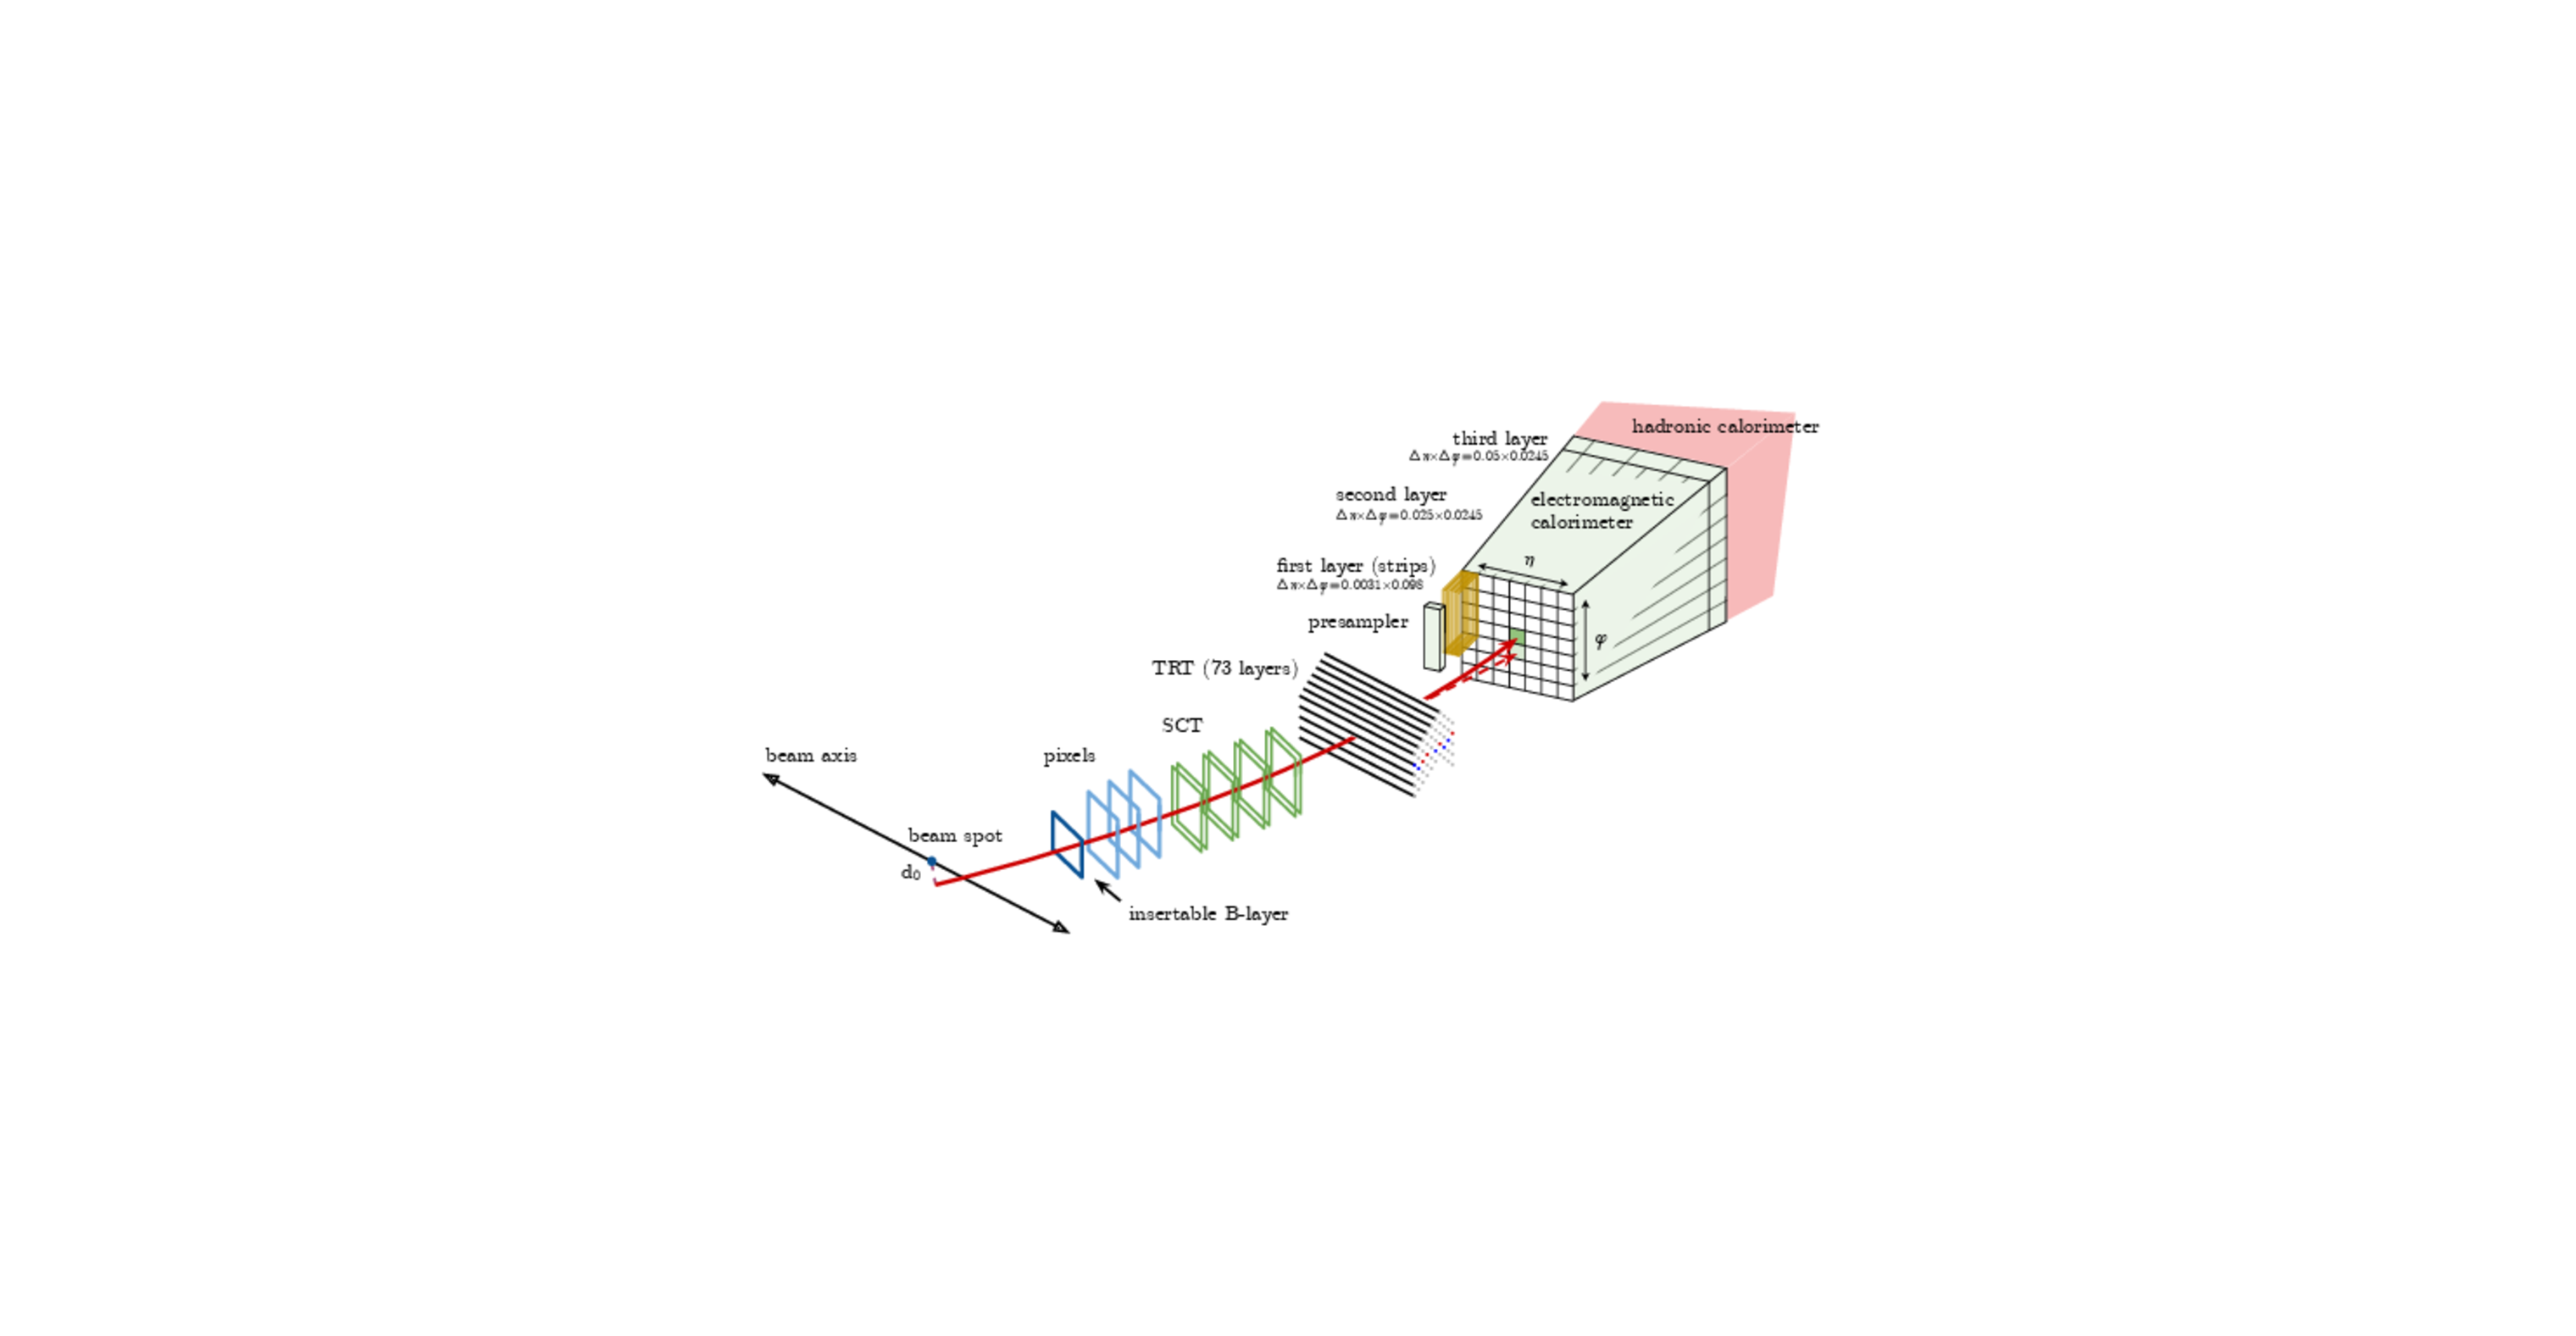
\includegraphics[width=0.80\textwidth,keepaspectratio]{figures/Reconstruction/electronPath}
\caption{
Schematics of the electron going through the detectors
}
\label{fig:electronPath}
\end{center}
\end{figure}
The electron candidate is from the area up to $|\eta|<2.47$, excluding the transition region between barrel and endcap (1.37 < $|\eta|$ < 1.52).
%identification
%The reconstructed electron is required the transverse energy of $E_T$ > 7~GeV and $|\eta|$ < 2.47. 
A likelihood-based identification (LHID) is required to reduce the backgrounds from photon conversion or hadron comes from jets. 
This LHID combines various identification variables, like shower shape of the ECal and the track conditions, and the matching of the tracks and the clusters.
The shower shape, or the ratio of the energy deposit in the hadronic calorimeter to that of the whole EM cluster can be used to separate the electrons from the light-flavour jets. The track conditions are useful to distinguish the electrons from photons.
Electron candidates are categorized to LooseLH, MediumLH, and TightLH corresponding to 96\%, 94\%, 88\% of identification efficiencies to signal electrons at $E_T$ = 100~GeV, respectively.
%put calibration things here.....
The reconstruction and identification efficiency is measured using  $J/\Psi \rightarrow ee$ and $Z\rightarrow ee$ and $Z\rightarrow ee\gamma$ events. The efficiencies are shown in Figure~\ref{fig:recoElectron}. The discrepancy between the data and the MC is corrected for using event-weight scale factors, parametrized with $E_T$ and $\eta$. Detailed information is in \cite{PERF-2017-01}.
%put momentum? resolutions here
\begin{figure}[tbp]
\begin{center}
%\subfigure[]{
 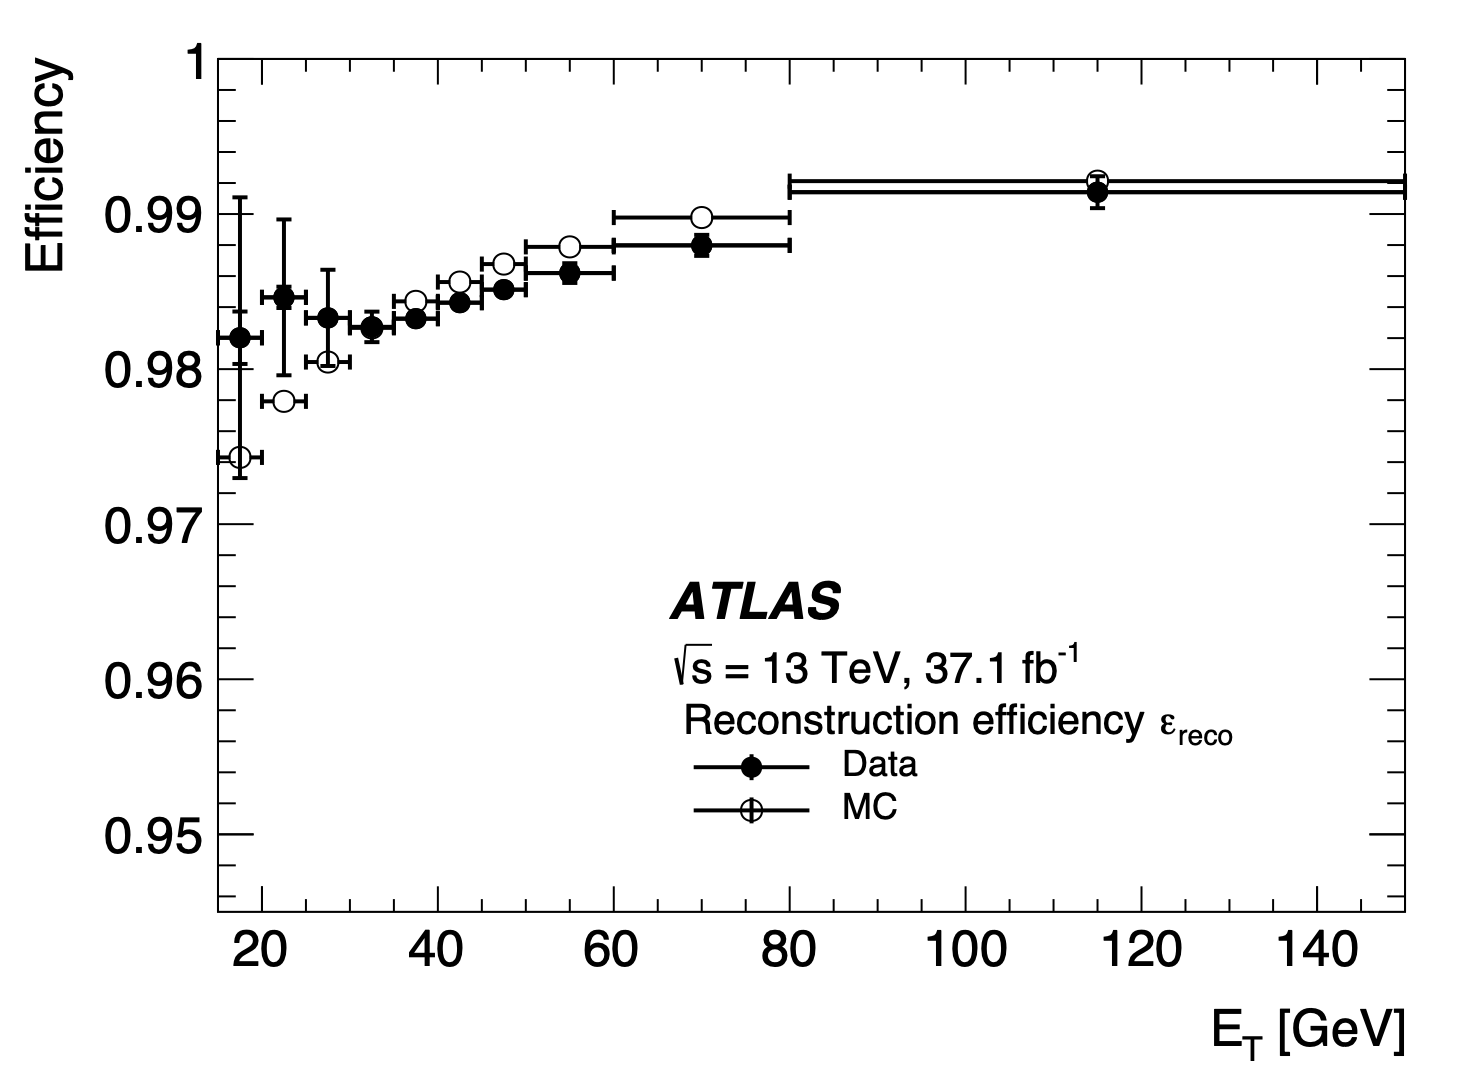
\includegraphics[width=0.50\textwidth,keepaspectratio]{figures/Reconstruction/recoElectron}
 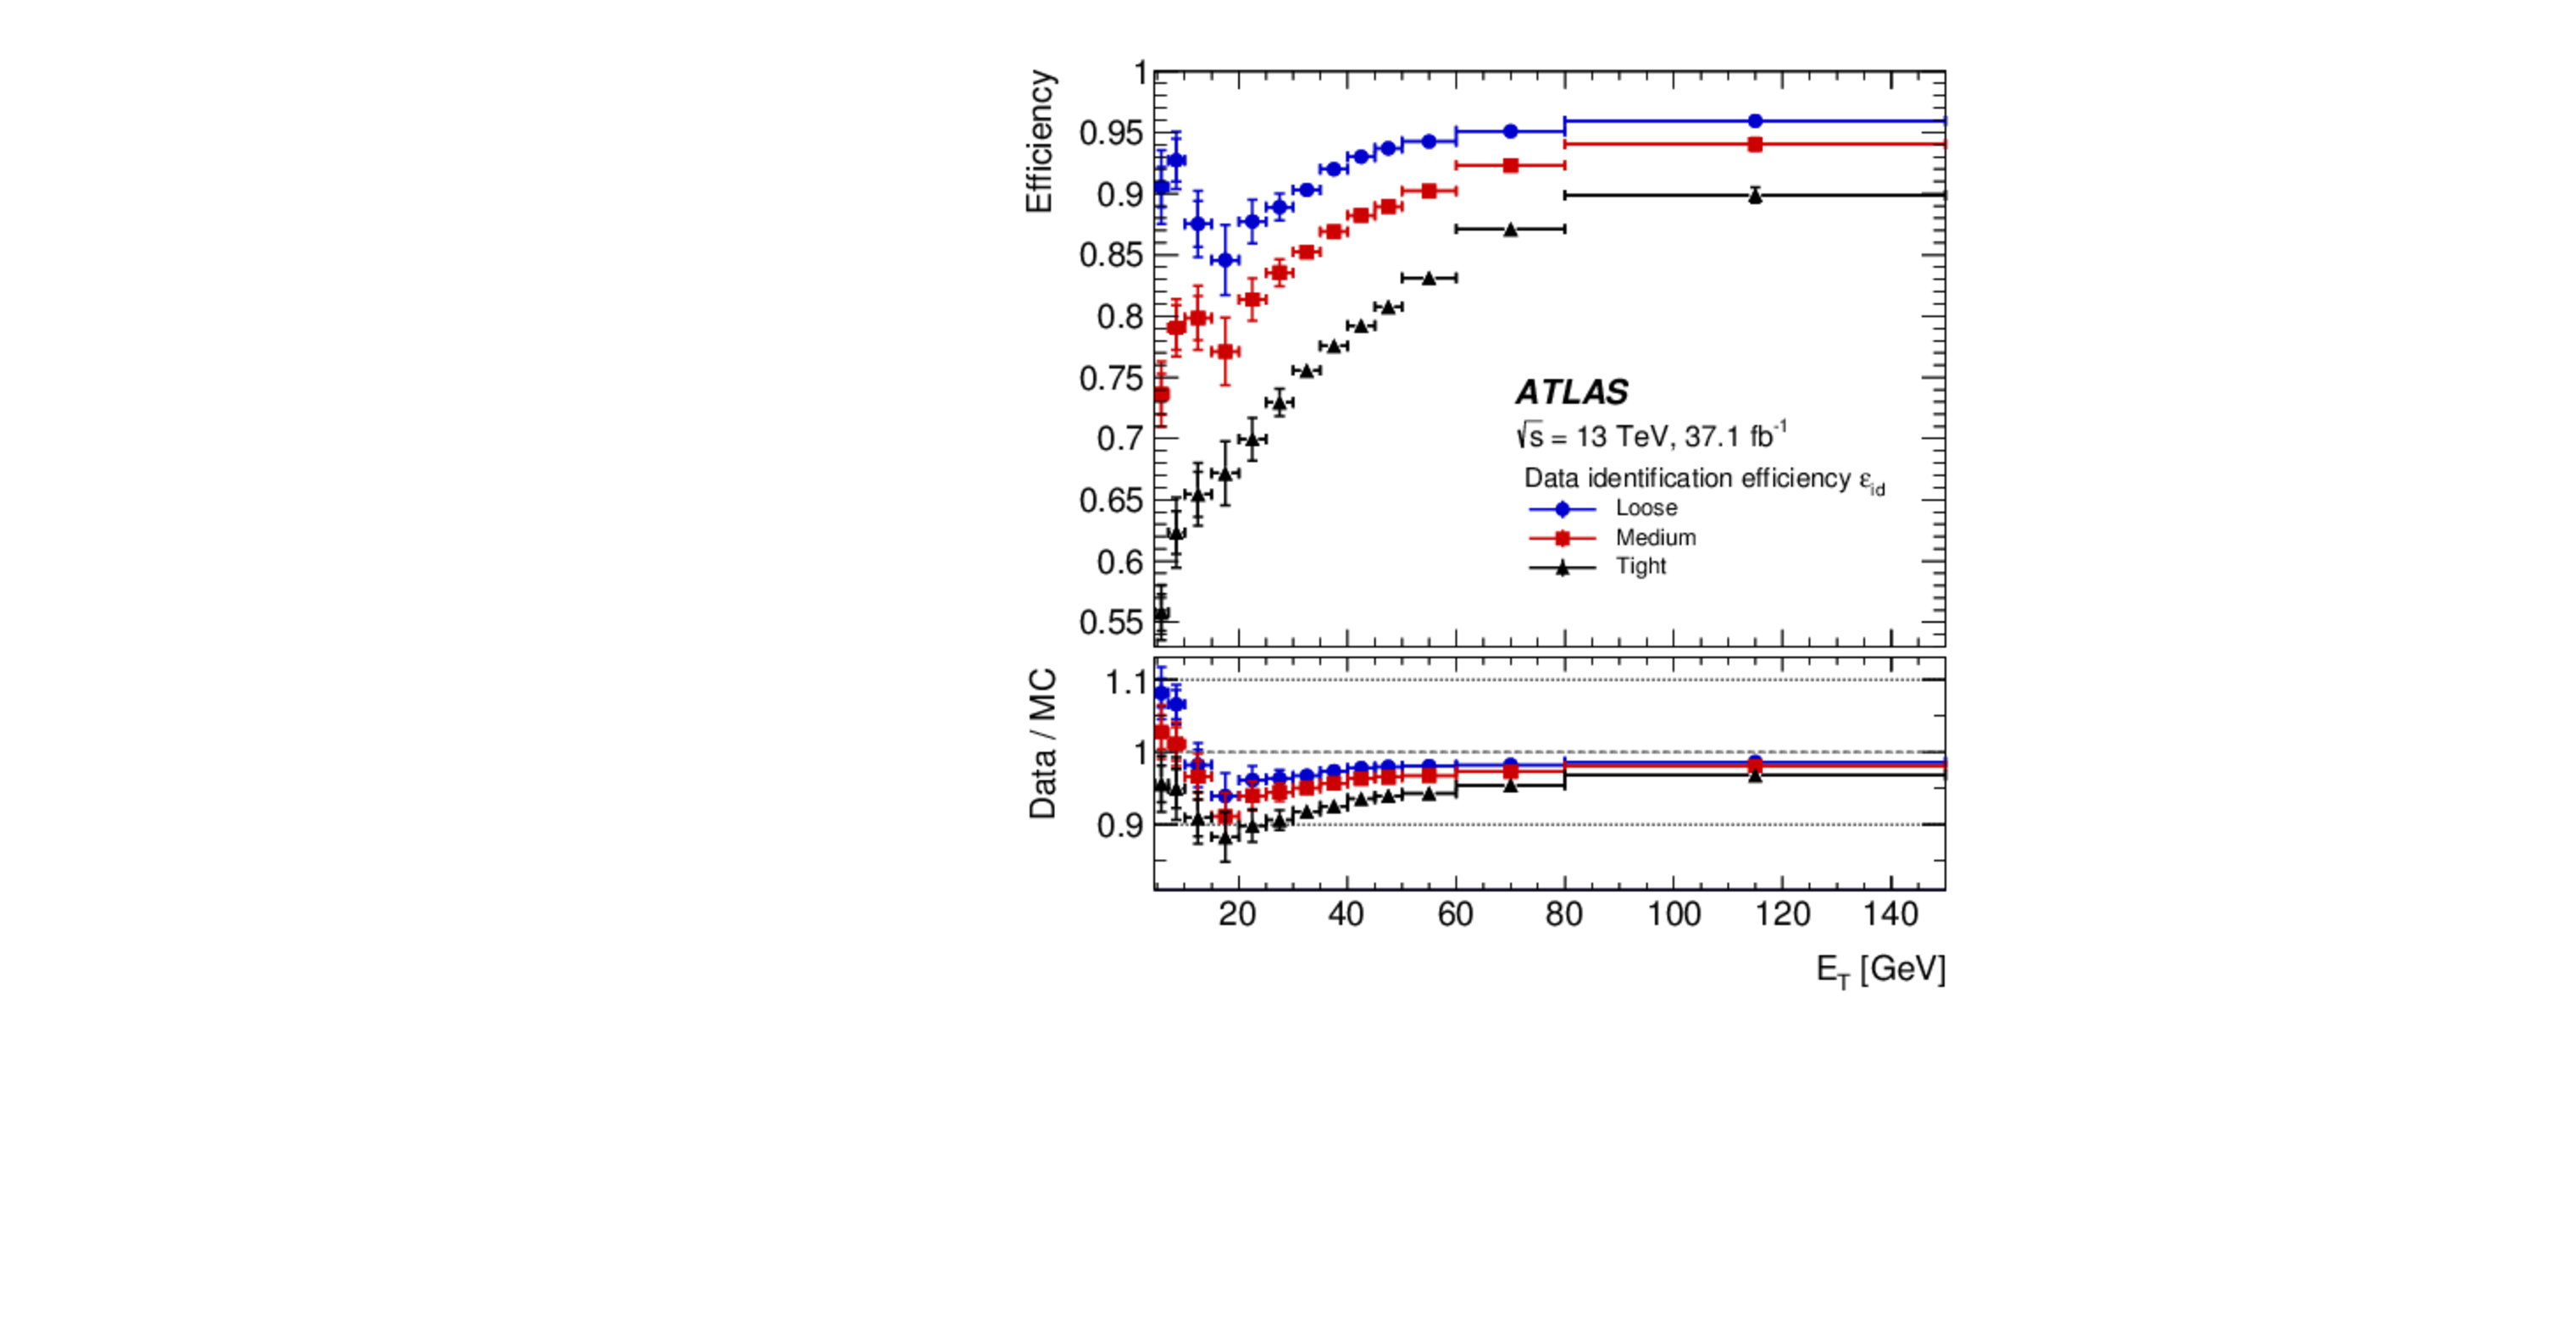
\includegraphics[width=0.45\textwidth,keepaspectratio]{figures/Reconstruction/idElectron}
%}
\caption{
electron reconstructing and identification efficiency with respect to the $E_T$
}
\label{fig:recoElectron}
\end{center}
\end{figure}
Several furthermore requirement is applied for isolation, to reduce the contamination with jets. The two isolation working points used in this analysis, which are determined by the track and ECal informations. The selections applied in this analysis are shown in the Table~\ref{tab:electron_selection}.
Furthermore, the track related requirement is applied. $d_0$ is a minimum distance between the primary vertex (PV) and the track, and $\sigma_{d_0}$ is its uncertainty. $z_0$ is the tranverse impact parameter relative to the beamline.
\begin{table}[ht]
\resizebox{0.8\textwidth}{!}{
\begin{tabular}[ht]{|l|c|c|c|}
  \hline
  & \emph{Loose} & \emph{Tight}\\
  \hline
  \hline
  $p_T$ & 7~GeV & 30~GeV\\
  \hline
  $|\eta|$ & \multicolumn{2}{c|}{$|\eta| < 2.47$ \notin [1.37,1.52]} \\
  \hline
  Identification & LooseLH & TightLH \\
  \hline
  Isolation &  FCLoose $(p_T <100~GeV)$                   &  FixedCutHighPtCaloOnly \\
            &  no isolation requirement $( >100~GeV )$ & \\
  \hline
  $|d_{0}/\sigma_{d_0}|$ & \multicolumn{2}{c|}{ <~5 }\\ 
  \hline
  $| z_{0} \sin{\theta}|$ & \multicolumn{2}{c|}{ <~0.5~mm }\\
  \hline
 \end{tabular}}
 \label{tab:electron_selection}
 \caption{Summary of electron selection used in this analysis}
\end{table}

\section{Muons}
%reconstruction
Muons reaches to the Muon Spectrometer (MS) as shown in Figure~\ref{}, and it is reconstructed by the combination of the tracks in the Inner Detector (ID) and Muon Spectrometer (MS). 
Figure~\ref{fig:recoMuon} shows the schematic diagram of the muon in the detectors.
%find and put the schematic of the muons
Several algorithm are used for the reconstruction: 
combined (CB) muons which require independent tracks both in ID and the MS. CB muons are of highest quality, but least acceptance. 
Segment-tagged (ST) muons require an ID track with only one hit in the MS, which allows recovering the low-$p_T$ muons. 
Calorimeter-tagged (CT) muon is reconstructed by requiring one ID track and in addition energy deposits in the calorimeter, which agree with a minimum-ionizing particle. CT muon are used to increase the acceptance in the region of $|\eta| < 0.1$, where the region without the muon cells due to the layout of the calorimeter cables. 
%reconstruction efficiency of calibration things
The muon reconstruction efficiency is measured with sample of $J/\Phi \rightarrow \mu\mu$ and $Z\rightarrow \mu\mu$, as well as the momentum scale and resolution.
The reconstruction efficiency is measured to be close to 99\% over most of the covered phase space ($|\eta|$ < 2.5 and 5 < $p_{T}$ < 100 GeV). The isolation efficiency varies between 93 and 100 \% depending on the selection applied and on the momentum of the muon. Both efficiencies are checked to be well reproduced in MC simulation. 
%In the central region of the detector, the momentum resolution is measured to be 1.7 \% (2.3 \%), and the momentum scale is known with an uncertainty of 0.05 \%. In the region $|\eta|$ > 2.2, the $p_T$ resolution for muons is 2.9 \% while the precision of the momentum scale for low-$p_T$ muons is about 0.2 \% \cite{}.
%identification
The further instructions are shown in \cite{MUON-2018-03}.
Similar to the electron, the isolation requirement is also applied to the muons, as shown in the Table~\ref{tab:muon_selection}.
\begin{figure}[tbp]
\begin{center}
%\subfigure[]{
 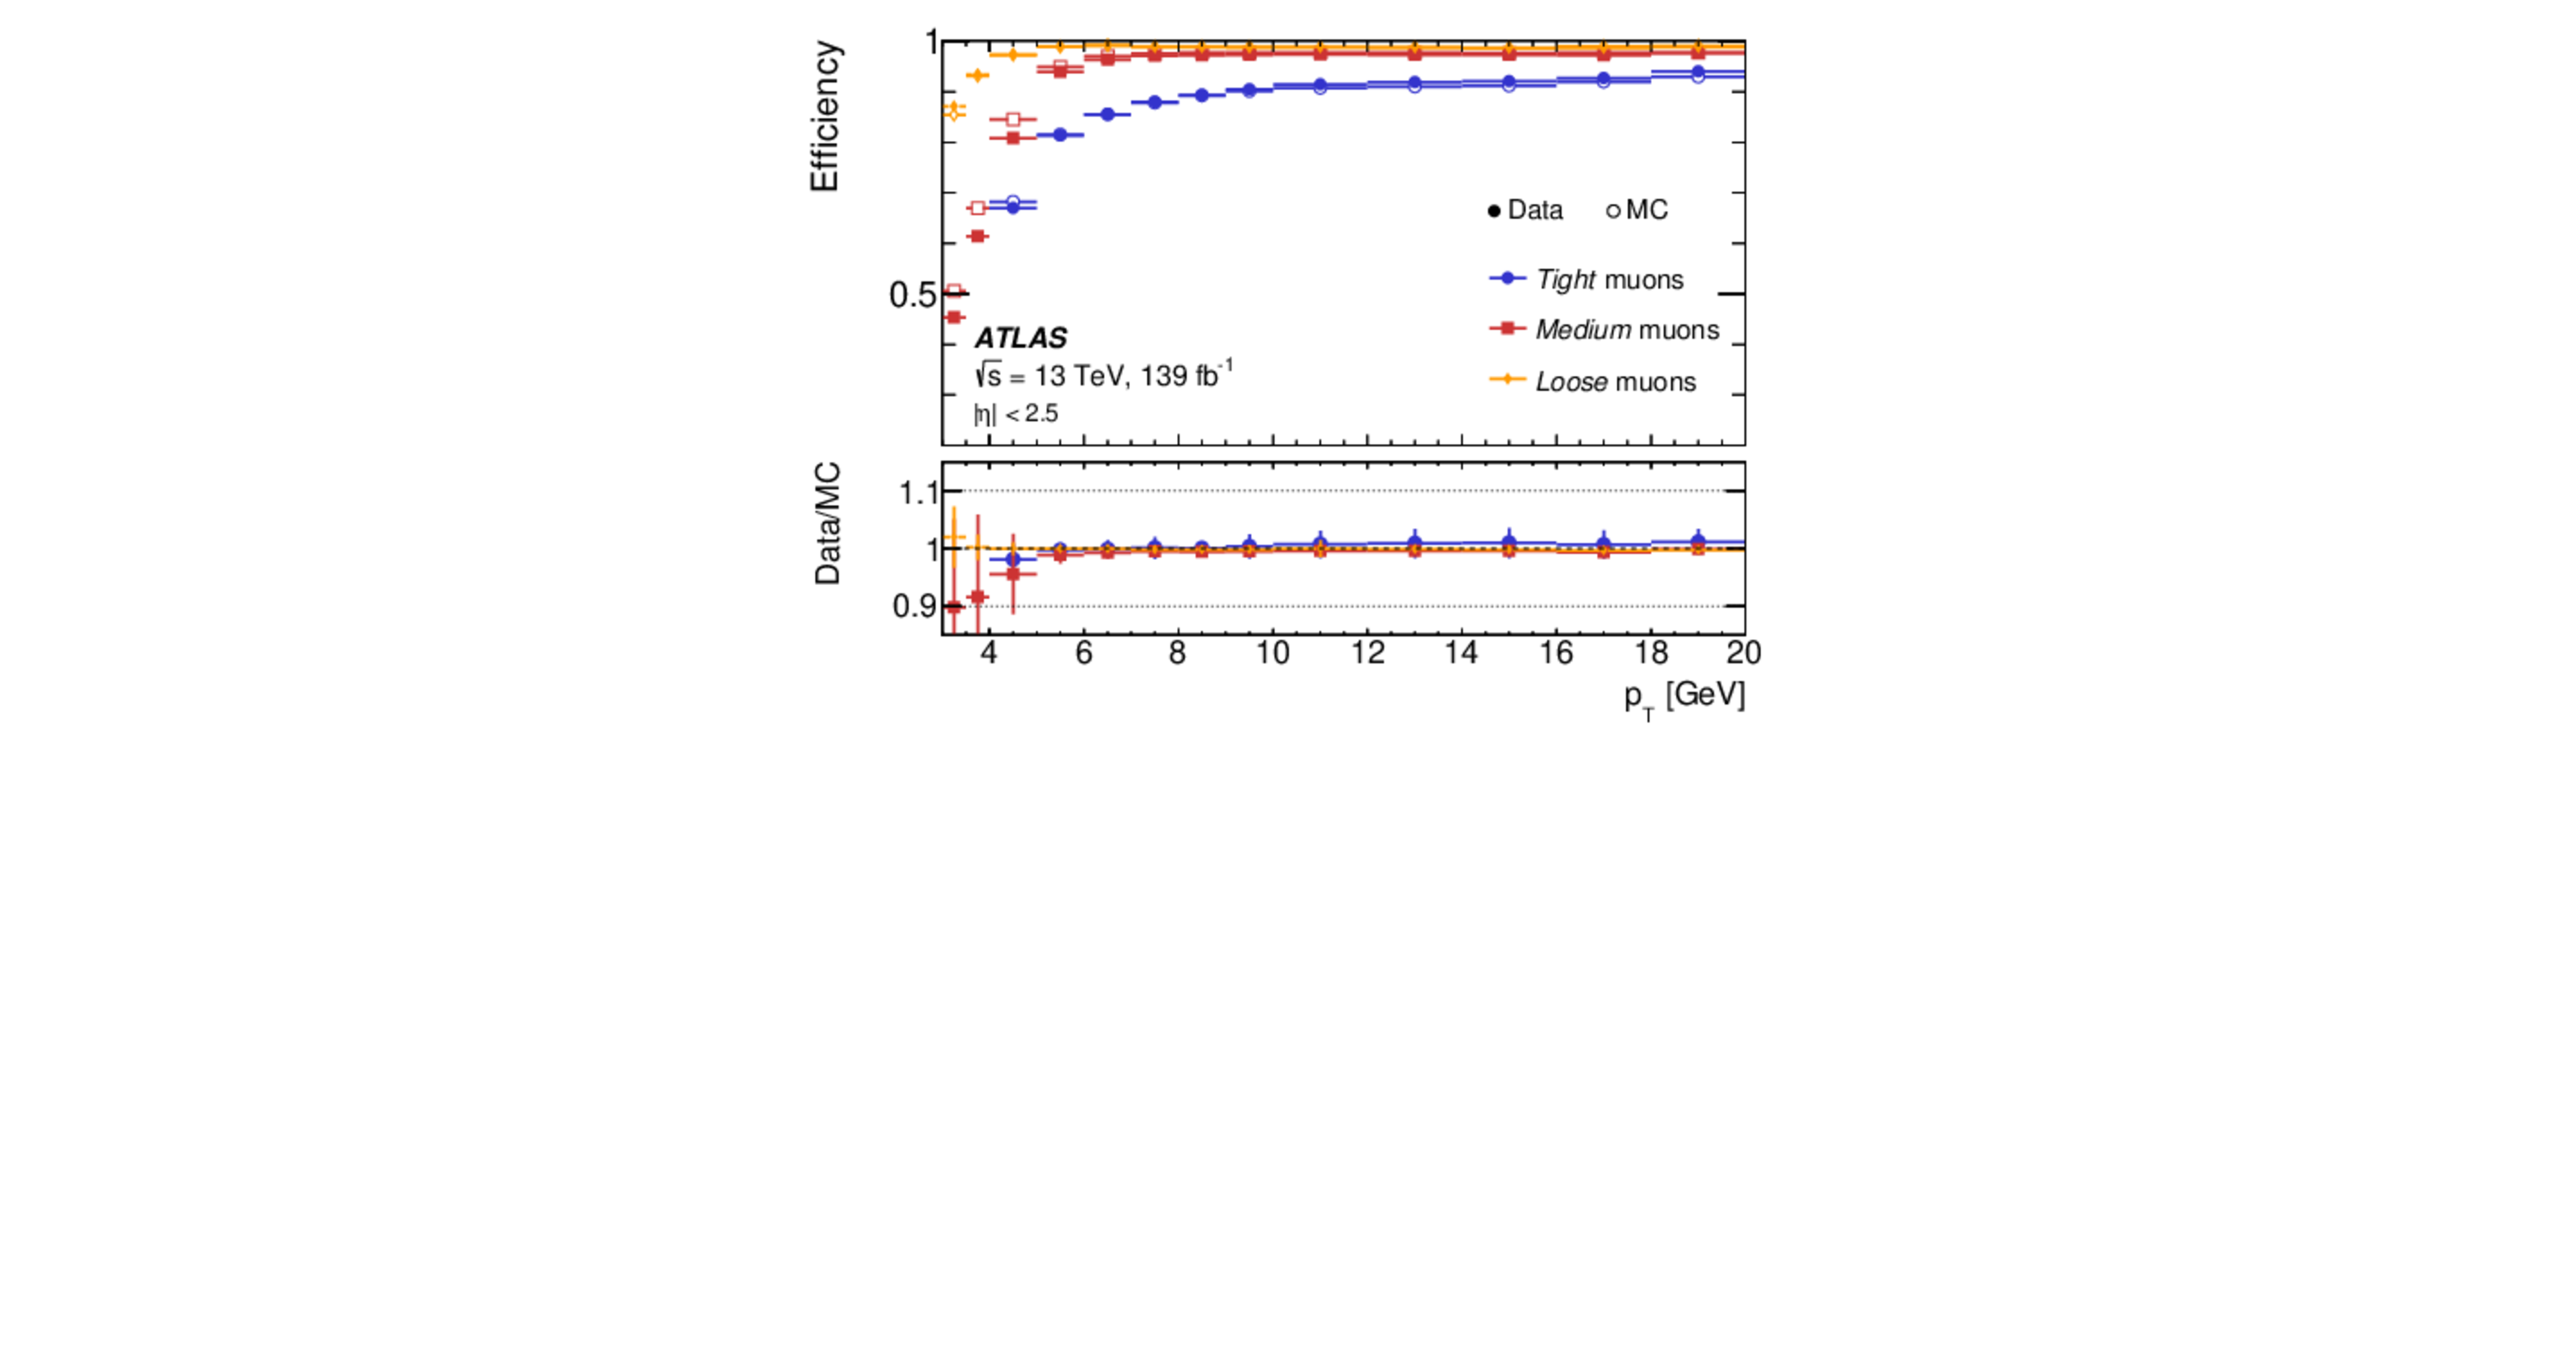
\includegraphics[width=0.45\textwidth,keepaspectratio]{figures/Reconstruction/recoMuonpT}
 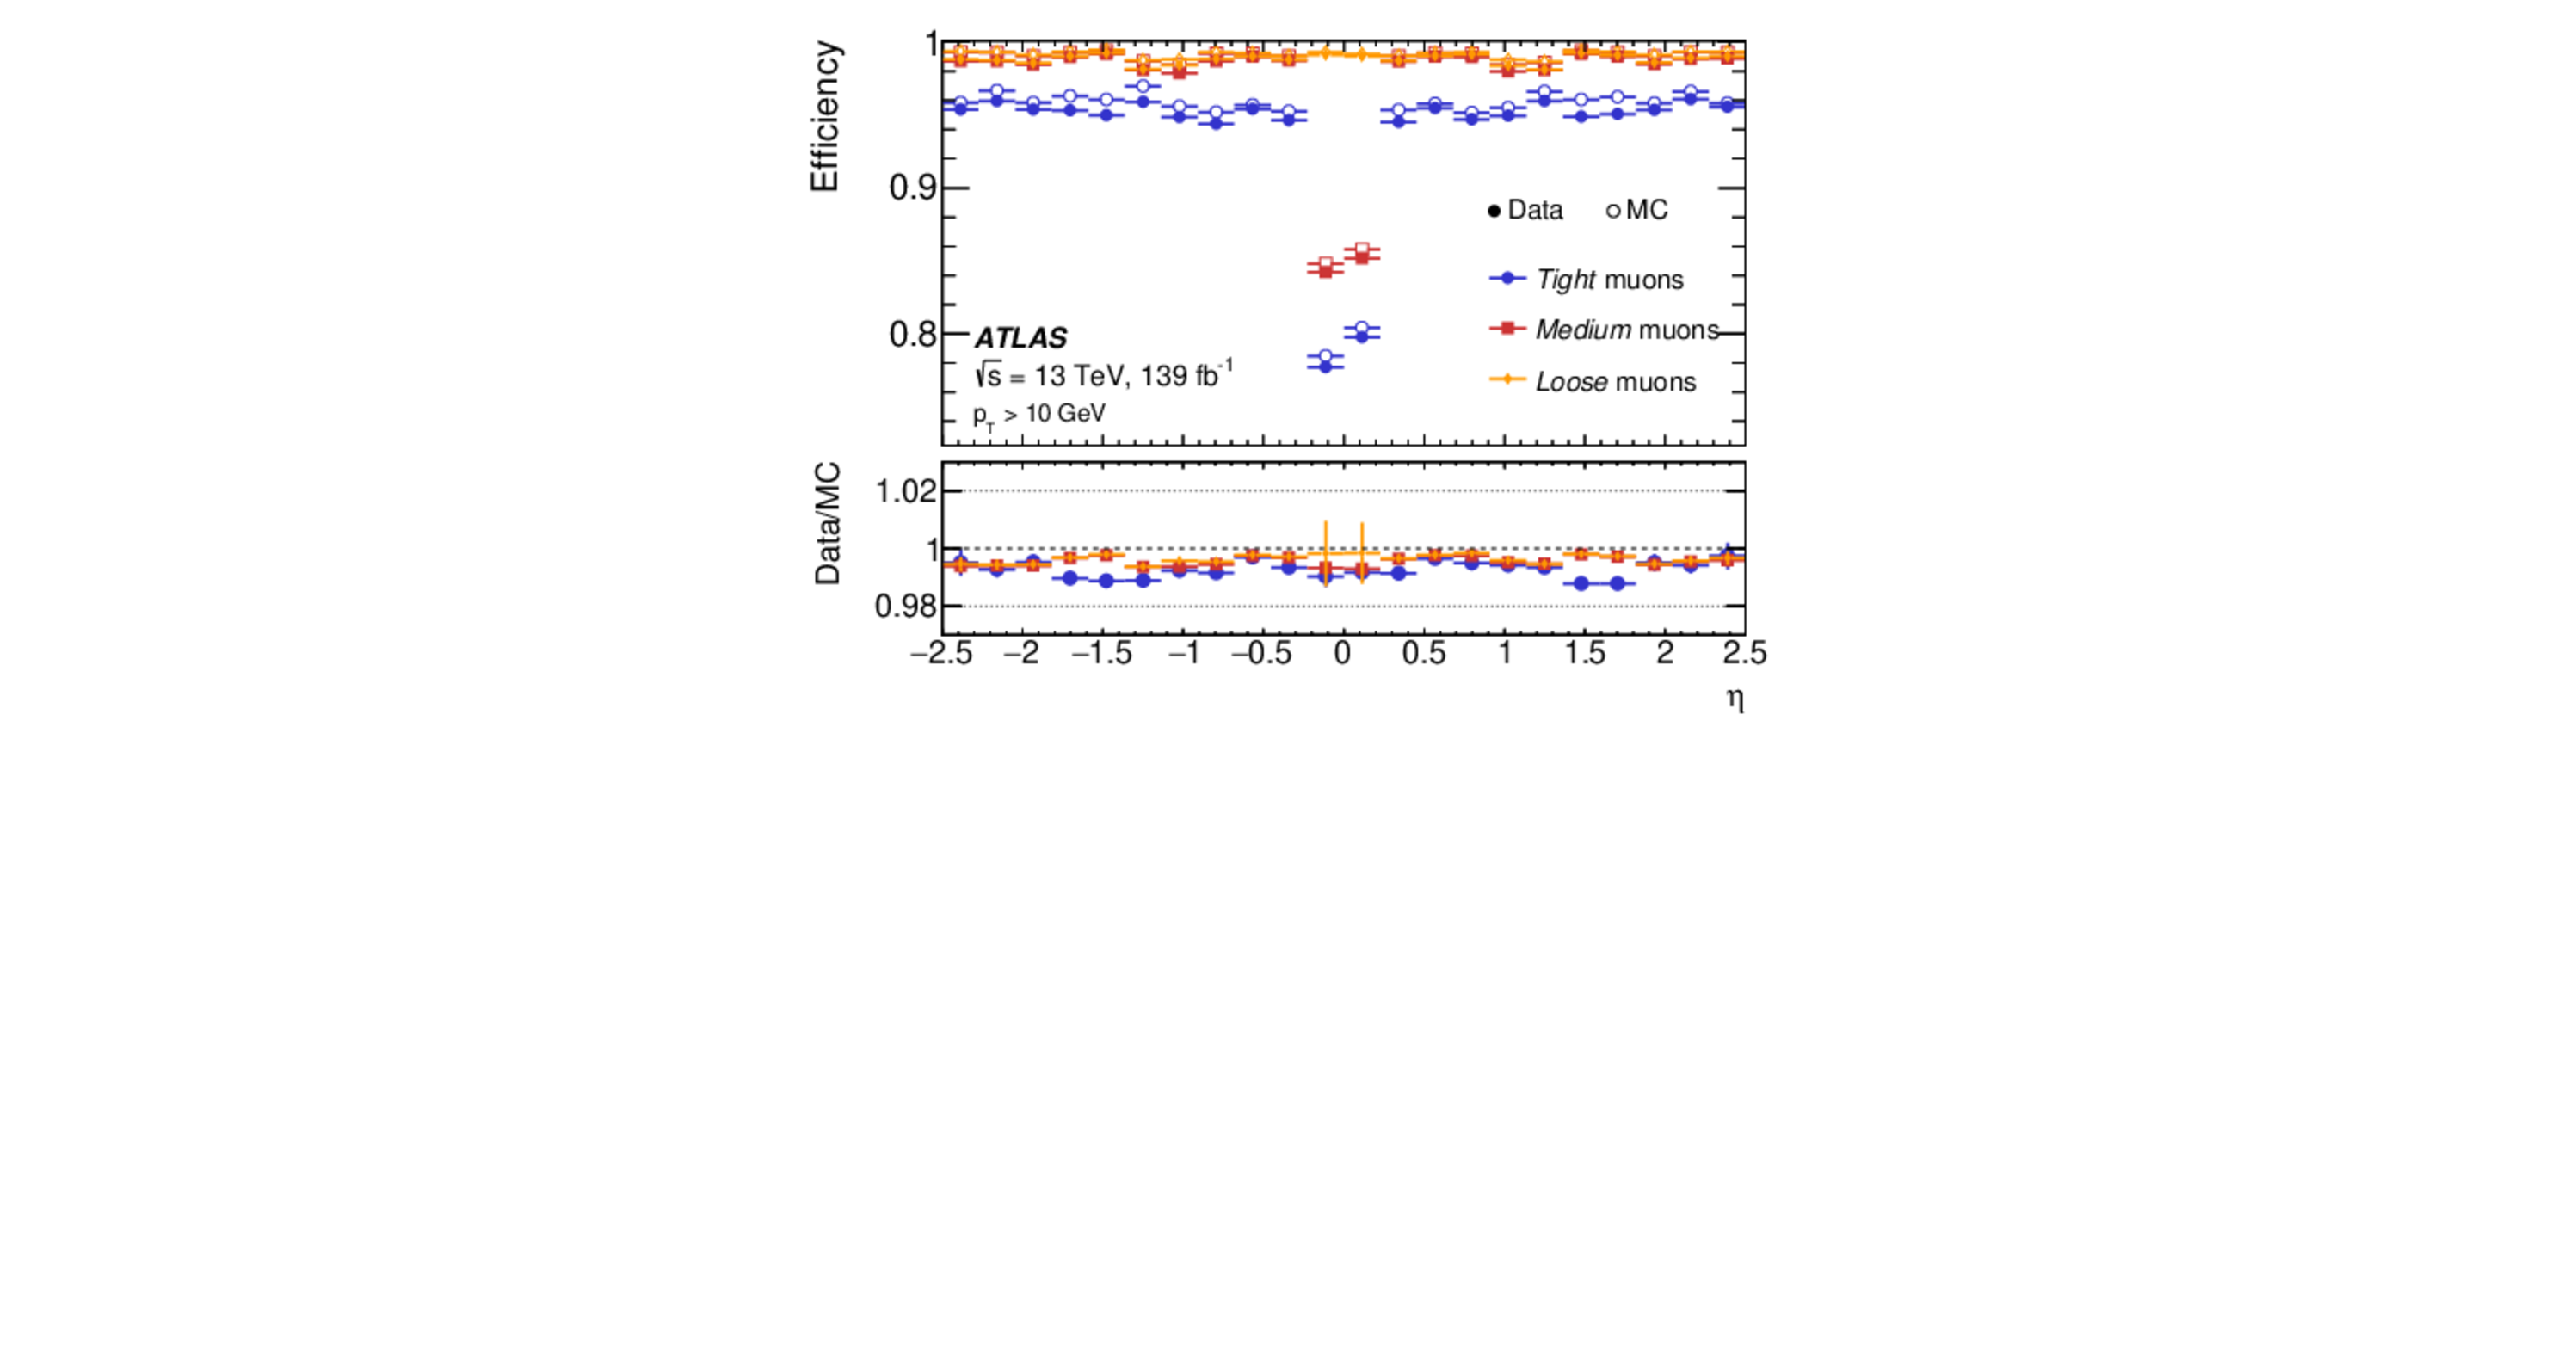
\includegraphics[width=0.45\textwidth,keepaspectratio]{figures/Reconstruction/recoMuonEta}
%}
\caption{
muon reconstructing and identification efficiency with respect to $E_T$ (left) and $eta$ (right) \cite{MUON-2018-03}
}
\label{fig:recoMuon}
\end{center}
\end{figure}
Muon identification is performed by applying quality requirements that suppress background, mainly from pion and kaon decays from the light-flavour jets. 
%It also selects prompt muons with high efficiency and/or guaranteeing a robust momentum measurement. 
For Medium muons, the CB tracks required to have more than three hits in at least two MDT layers exept for |$\eta$|<0.1.
Specifically, the q/p significance, defined as the absolute value of the difference between the ratio of the charge and momentum of the muons measured in the ID and MS divided by the sum in quadrature can be used for distinguish the muons.It is required to be less than seven for the contamination of the hadrons misidentified as muons.
The Loose identification uses all types of Muons. All CB and ME muons satisfying the Medium requirements are included. 
The identification used in this analysis is shown in Table~\ref{tab:muon_selection}.
\begin{table}[ht]
\resizebox{0.8\textwidth}{!}{
\begin{tabular}[ht]{|l|c|c|c|}
  \hline
  & \emph{Loose} & \emph{Tight}\\
  \hline
  \hline
  $p_T$ & 7~GeV & 30~GeV\\
  \hline
  $|\eta|$ & \multicolumn{2}{c|}{$|\eta| < 2.5$} \\
  \hline
  Identification & Loose & Medium \\
  \hline
  Isolation &  FCLoose $(p_T <100~GeV)$                   &  FixedCutHighPtCaloOnly \\
            &  no isolation requirement $( >100~GeV )$ & \\
  \hline
  $|d_{0}/\sigma_{d_0}|$ & \multicolumn{2}{c|}{ <~3 }\\ 
  \hline
  $| z_{0} \sin{\theta}|$ & \multicolumn{2}{c|}{ <~0.5~mm }\\
  \hline
 \end{tabular}}
 \label{tab:muon_selection}
 \caption{Summary of muon selection used in this analysis}
\end{table}

\section{Jets}
Hadrons can be seen as jets as the results of hadronization, as described in Section~\ref{}.
These are detected in the detector at the calorimeters as shown in Figure~\ref{fig:ParticlePath}.
Jets are basically reconstructed by grouping energy deposits in the calorimeter into clusters. These are then combined by the anti-$k_t$ algorithm \cite{Cacciari_2008}, with a radius of R = 0.4 (small-R jets) or R = 1.0 (large-R jets). The small-R jet contains most of the radiation from the quark or gluon jets. The large-R jets represents the hadronic decays of the heavy, boosted objects like W, Z bosons.

The anti-$k_t$ algorithm defines a measure of distance $d_{ij}$ between clusters in the calorimeter,
\begin{equation}
d_{i j}=\min \left\{\frac{1}{k_{\mathrm{T}, i}^{2}}, \frac{1}{k_{\mathrm{T}, j}^{2}}\right\} \times \frac{\left(\Delta R_{i j}\right)^{2}}{R^{2}}
\end{equation}
where $k_{T,i}$ is the transverse momentum of cluster i and $\Delta R_{i j}=\sqrt{\left(\Delta y_{i j}\right)^{2}+\left(\Delta \phi_{i j}\right)^{2}}$ is the distance between clusters i and j with y being the rapidity. Then search the minimum $d_{i j}(k)$ combinations. if $d_{i j}(k) = d_{i B}(k)$, cluster i is regarded as a jet otherwise cluster i and j are grouped together and the recalculate minimum distance. This procedure is repeated until all clusters are grouped into jets.
Figure~\ref{fig:antikt} shows how the clustering performed for example.
\begin{figure}[tbp]
\begin{center}
%\subfigure[]{
 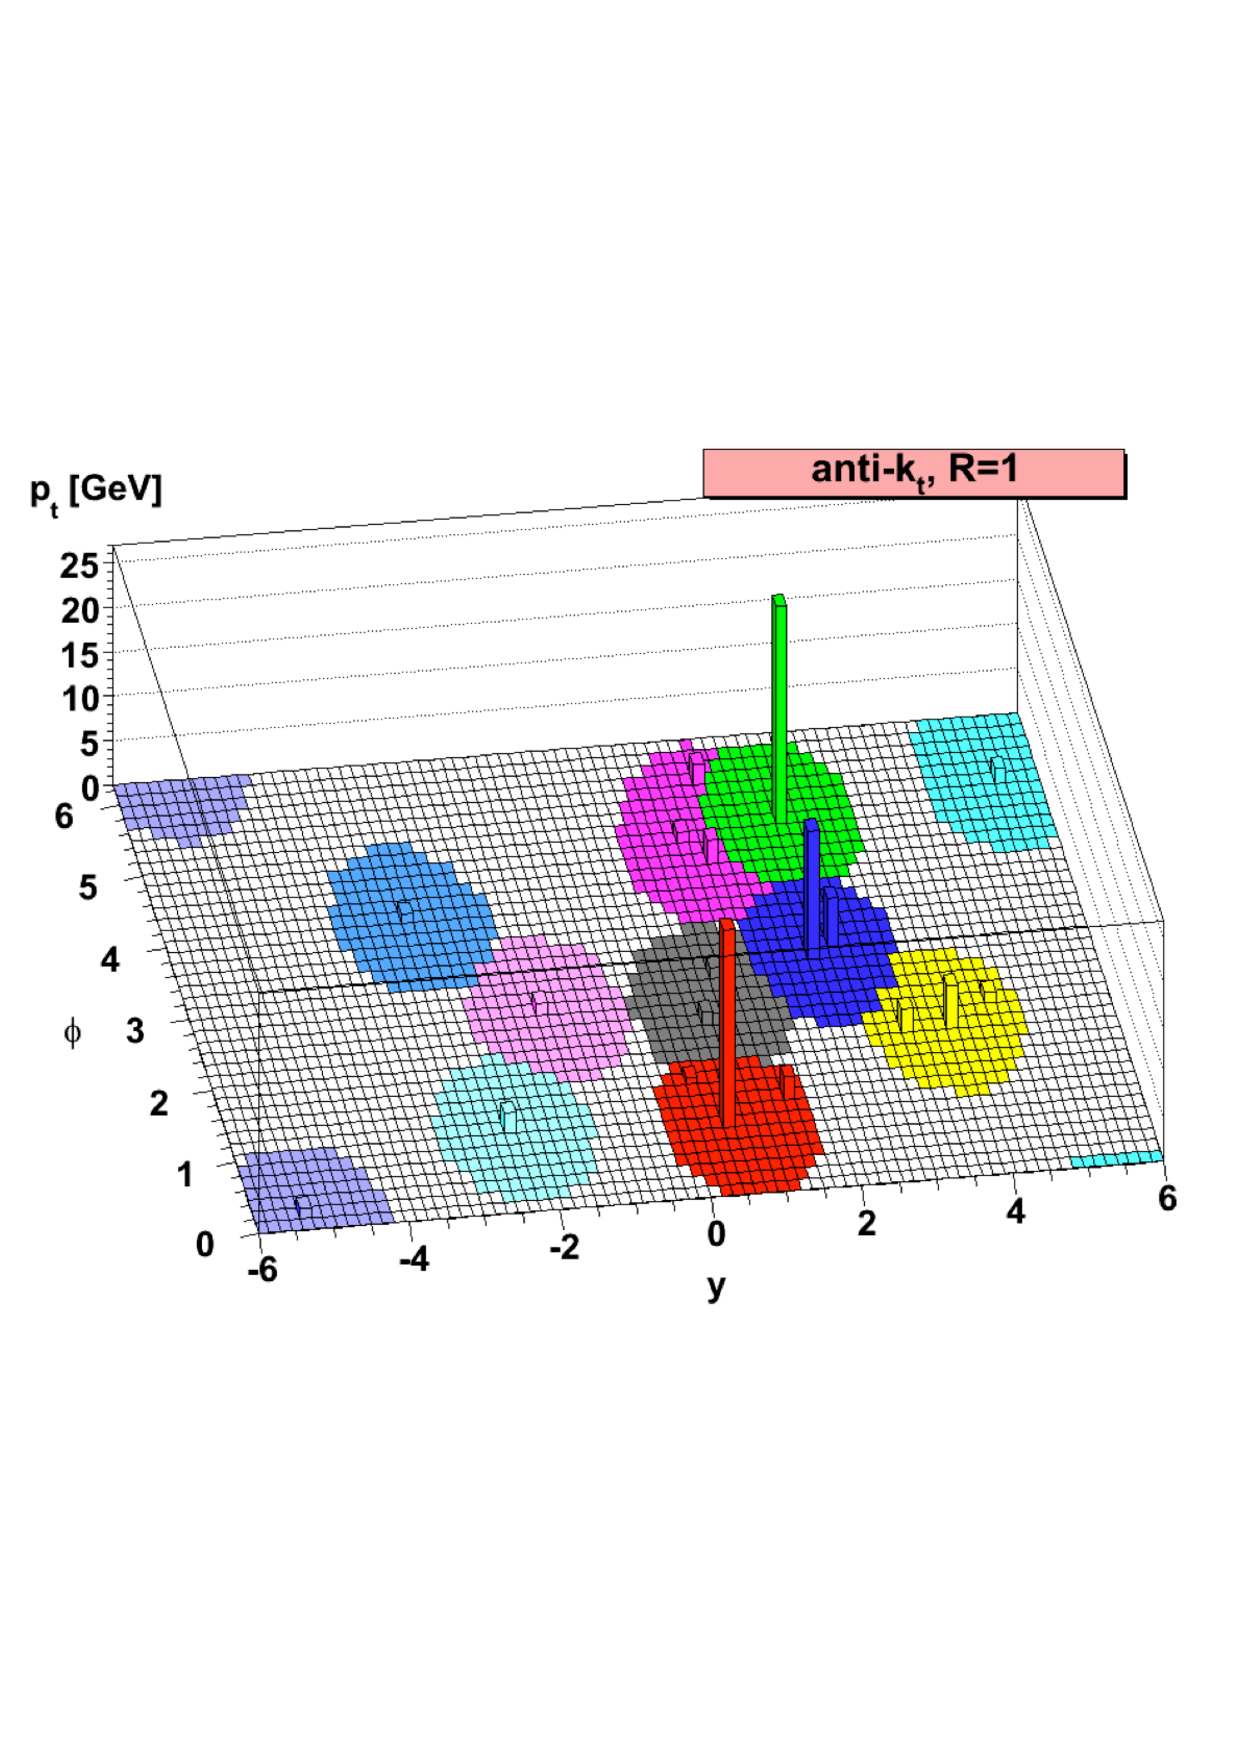
\includegraphics[width=0.70\textwidth,keepaspectratio]{figures/Reconstruction/antikt}
\caption{
anti-$k_T$ algorithm \cite{Cacciari_2008}
}
\label{fig:antikt}
\end{center}
\end{figure}

\subsection{small-R Jets}
The small-R jets are reconstructed with the topo-clusters using anti-$k_T$ algorithm with R = 0.4. In order to give better performance of measuring the energy and the momentum of the hadronic jets, particle flow algorithm \cite{PERF-2015-09} is adopted. The algorithm uses the ensemble of signals from the calorimeter and the inner tracker. 

The ID tracker information has better resolution for low-$p_T$ particles, and better angular resolution and can trace the particles to hard-scatter
interaction or pile-up. On the other hand, Carolimeters have better resolutions for high $p_T$ and can get neutral particles. Therefore the combined information can improve energy and angular resolution, as well as reduce the pile-up contributions.
%put somewhere the description about pile-ups
First tracks from the ID are selected, then the tracks to corresponding topo-clusters are matched. Second energy from the cluster depending on tracks position and $p_T$ is subtracted, and the tracks and remaining topo-clusters constitute the PFlow objects are selected.

%calibration
The calibration for the jets are done with several steps in order to do the correction for all detector effects. 
\begin{itemize}
    \item pileup-substruction \\
    The per-event pileup contributions to the $p_T$ of each jets are removed based on each area. It is subtracted based residual $N_{PV}$ and $\mu$ (average interaction per crossing) \cite{JETM-2018-05}.
    The corrected jet $p_T$ is described as:
    \begin{equation}
     p_{T}^{\text {corr }}=p_{T}^{\text {reco }}(-\rho \times A)-\alpha\left(N_{P V}-1\right)-\beta\langle\mu\rangle
    \end{equation}
    This correction with repect to $\eta$ is shown in Figure~\ref{fig:pileup}.
    \begin{figure}[tbp]
    \begin{center}
    %\subfigure[]{
    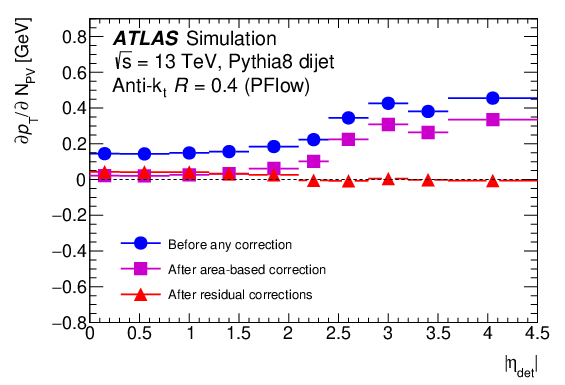
\includegraphics[width=0.45\textwidth,keepaspectratio]{figures/Reconstruction/intimepileup}
    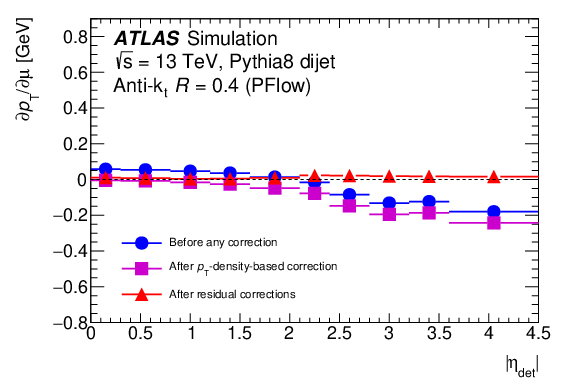
\includegraphics[width=0.45\textwidth,keepaspectratio]{figures/Reconstruction/outtimepileup}
    \caption{
    pile-up subtraction \cite{JETM-2018-05}
    }
    \label{fig:pileup}
    \end{center}
    \end{figure}
    \item JES, $\eta$, mass calibration \\
    The detector responses are different across detector, especially at the boundaries between calorimeter technology and the granualarities. Some corrections are applied as function of E and $\eta$, by comparing the reconstructed jets to truth jets (energy response, $\mathrm{E}^{\text {reco }} / \mathrm{E}^{\text {truth }}$ ) which derived from the truth MC \cite{JETM-2018-05}.
    Figure~\ref{fig:JES} shows the jet energy response as a function of $\eta$.
    \begin{figure}[tbp]
    \begin{center}
    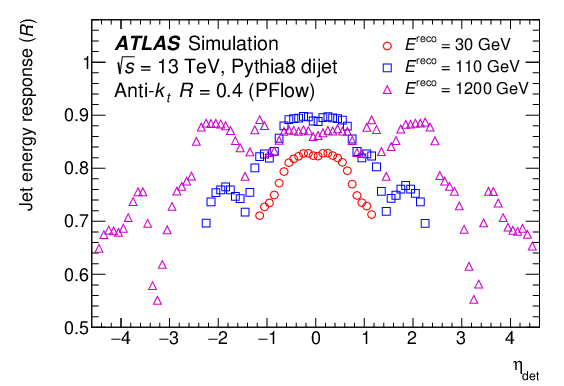
\includegraphics[width=0.60\textwidth,keepaspectratio]{figures/Reconstruction/JES}
    \caption{
    Jet energy response \cite{JETM-2018-05}
    }
    \label{fig:JES}
    \end{center}
    \end{figure}
    \item Global sequential calibration \\ %?? these are for large-R jets?
    The Global Sequential Calibration (GSC) is applied, mainly to accounting for the different response to quark and gluon initiated jets. It also includs the correction for the punch-through, which is jets with large $p_T$ whose energy is not fully contained in calorimeter \cite{JETM-2018-05}.
    \item In-situ validation \\
    The last calibration step is a correction with respect to the data. This is a adjustment for potential difference between data and MC, and this is only applied to the data.
    This calibration uses methods which rely on well-calibrated reference objects in the event to constrain the jet $p_T$ response. 
    Sets of the measurements are combined to give a continuous calibration curves of the ratio of the jet response as a function of jet $p_T$, shown in Figure~\ref{fig:in-situcalibration}.
    \begin{figure}[tbp]
    \begin{center}
    %\subfigure[]{
    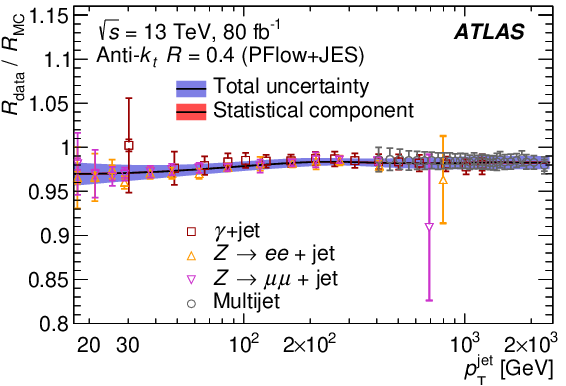
\includegraphics[width=0.6\textwidth,keepaspectratio]{figures/Reconstruction/insitucalibration}
    \caption{
    in-situ calibration \cite{JETM-2018-05}
    }
    \label{fig:in-situcalibration}
    \end{center}
    \end{figure}
\end{itemize}
The total jet energy scale uncertainty with respect to these calibration is shown in Figure~\ref{fig:allJES}.
\begin{figure}[tbp]
    \begin{center}
    %\subfigure[]{
    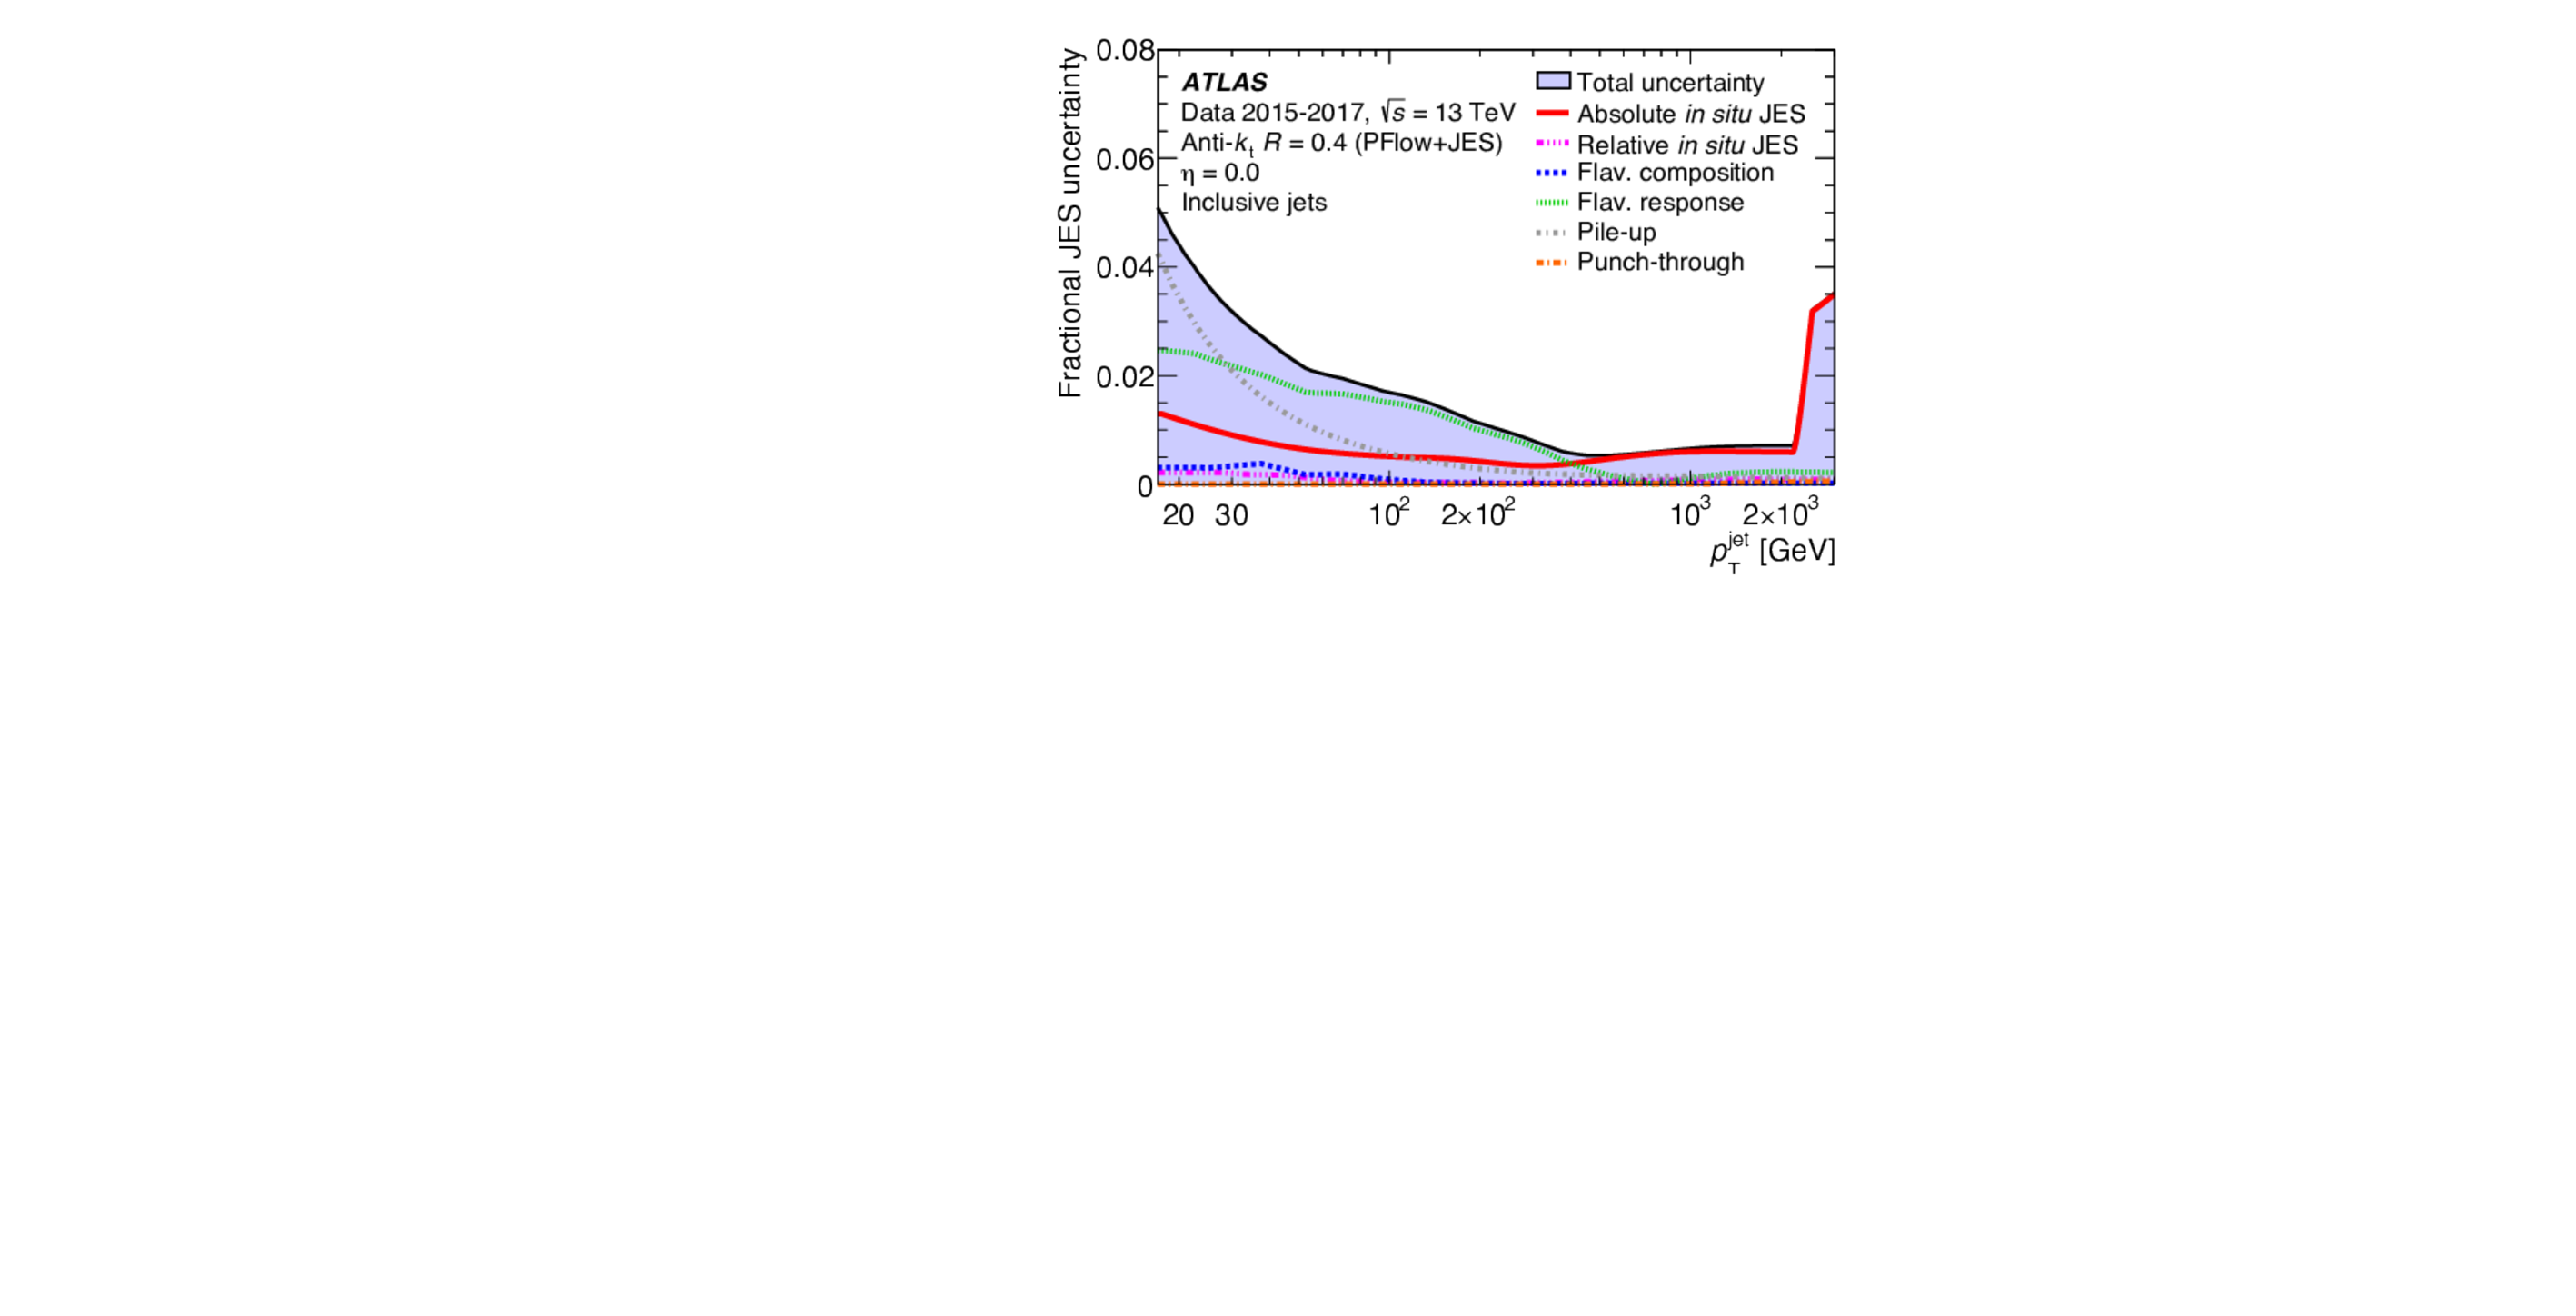
\includegraphics[width=0.6\textwidth,keepaspectratio]{figures/Reconstruction/allJES}
    \caption{
    All JES-related uncertainties is shown in black line. \cite{JETM-2018-05}
    }
    \label{fig:in-situcalibration}
    \end{center}
\end{figure}
%identification

The small-R jets are required to be $p_T$ > 20~GeV ($|\eta|$<2.5) and > 30~GeV (2.5 < $|\eta|$ < 4.5).
The jet vertex tagger (JVT) is applied to identify the jets only from the hard interaction. Furthermore, in the context of the pile-up suppression, forward jet vertex tagger (fJVT) has been introduced, motivated by the forward-like topology in this analysis.
The b-tagging is used for rejecting the jets tagging as including the b-hadrons, to suppress the top contributions.

\subsubsection{JVT}
\subsubsection{fJVT}

\subsubsection{B-tagging}
The small-R jets containing a b-hadron are identified by DL1r algorithm~\cite{ATL-PHYS-PUB-2020-009}, using a deep-learning neural network.
%The DL1r b-tagging is based on the features of b-hadrons in terms of the impact parameter of tracks and the displaced vertices reconstructed in the inner detector.
The Dl1r combines four low-level tagger, IP3D~\cite{ATL-PHYS-PUB-2017-013}, SV1~\cite{ATL-PHYS-PUB-2017-011}, JetFitter~\cite{ATL-PHYS-PUB-2018-025}, and RNNIP~\cite{ATL-PHYS-PUB-2017-003}.
The so-called b-tagging algorithm is used to distinct b jets from c jets or light jets, which initiated by c-quarks or gluons,u,d,s quarks respectively.
The lifetime of the b hadrons are long enough to travel several mm from the primary interaction before decaying, and create secondary vertices. These can be reconstrcuted using the tracks from the inner detector.
The IP3D uses signed impact parameter significance. The impact parameter, $d_0$ denotes the distance between tracks and the primary vertex as shown in Figure~\ref{fig:bdecay}.
The SV1 reconstructs the secondary vertex in a jets. The JetFitter reconstructs the topology of b/c-hadron decay chains using Kalman filter~\cite{FRUHWIRTH1987444}.
Additionally, the RNNIP uses the track features including the track quality informations.
At last the DL1r combines the outcomes all of these four low-level tagger by deep-learning neural network algorithm.
%The DL1r output and the efficiency of the b-tagging using DL1r are shown in Figure~\ref{}.
In this analysis the b-tagging working point is fixed at 70\% efficiency.

\subsection{large-R Jets}
large-R jets are reconstructed with topo-cluster using anti-$k_T$ algorithm similar to the small-R jets but with R = 1.0. The calibration applied for the large-R jets are mainly same as the procedure with the small-R jets, described in subsection~\ref{}, though there are some specific calibrations for large-R jets.

What is specific to the large-R jet is that the reconstructed topo-clusters are highly contaminated by the calorimeter nose and the 
\begin{itemize}
    \item Grooming \\
    Grooming techniques reduce contributions from pile-up and soft and wide angle emmissions.
\end{itemize}

\subsection{Vector Boson Identification}



%%%%%%
\section{Missing Transverse Momentum}


